% Tests
\chapter{Tests}

\section{Open-Loop Pointing Test}
\begin{figure}[!htb]
  \begin{minipage}{.49\textwidth}
    \centering
    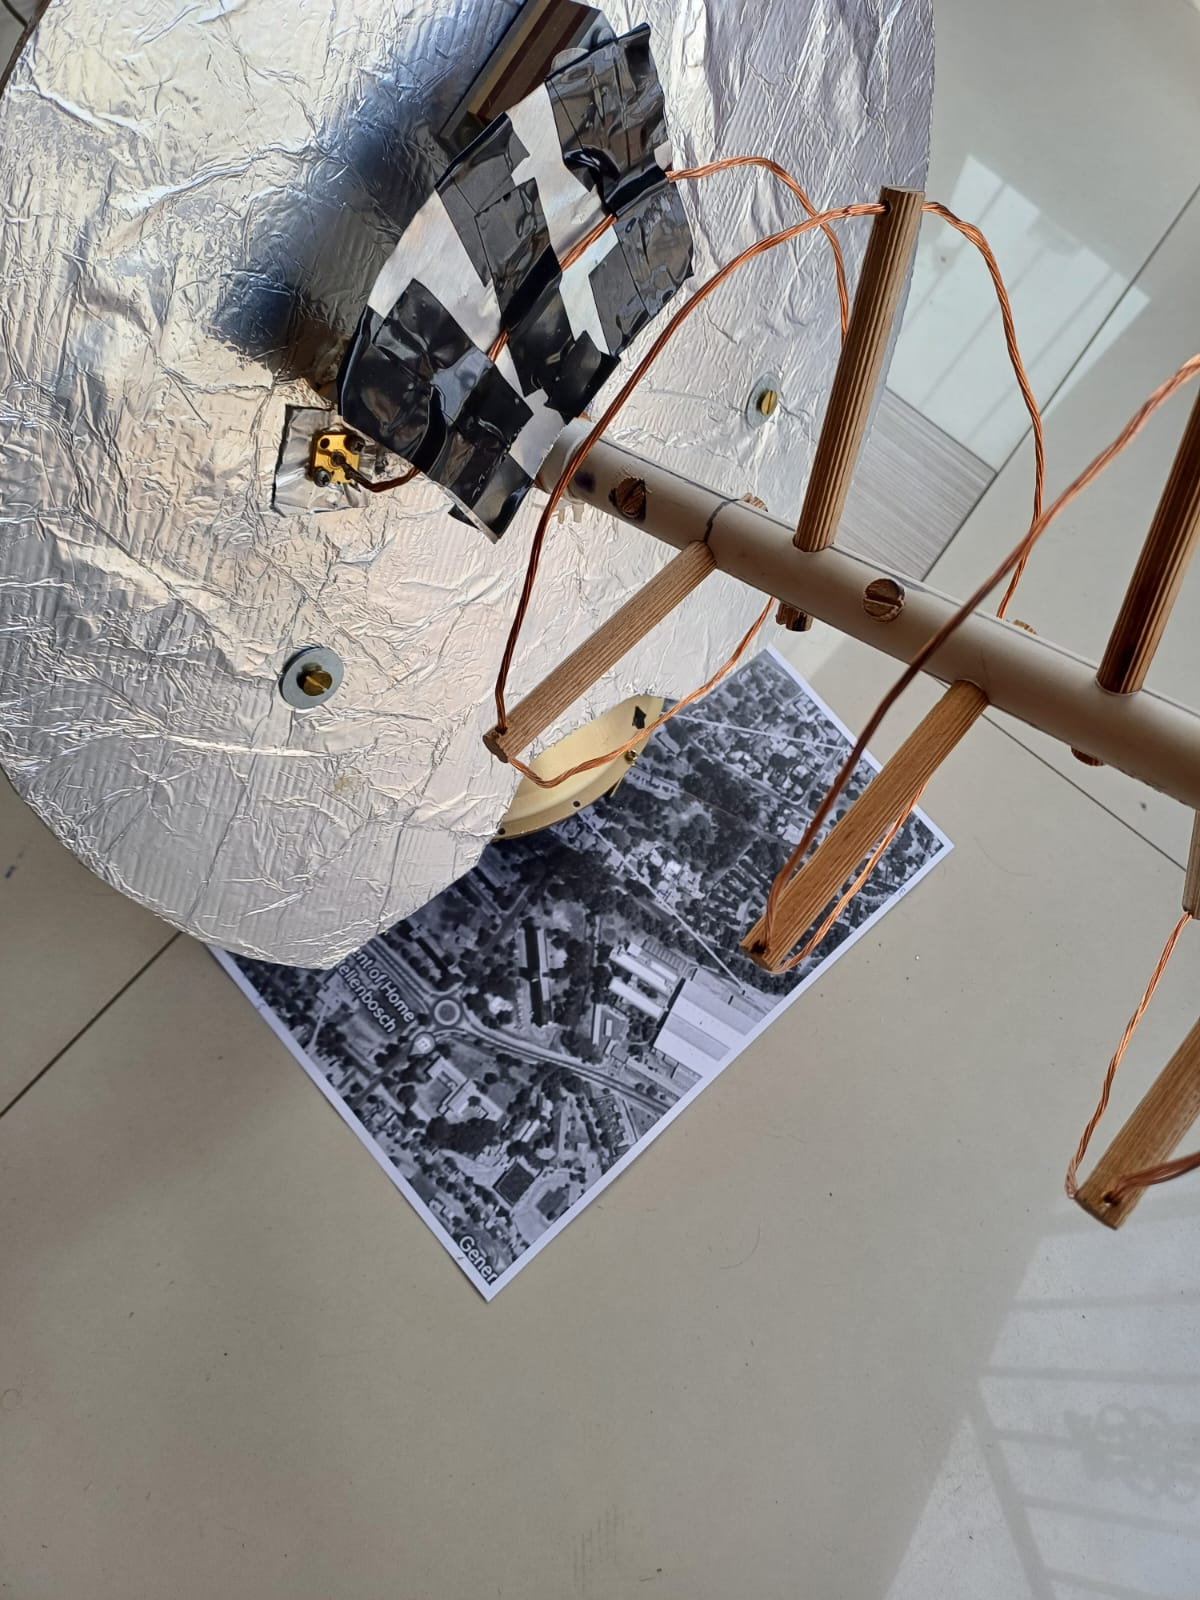
\includegraphics[width=0.8\linewidth]{pointingTestSetup}
    \caption{Open-Loop Pointing Test Setup}
    \label{fig:pointingTestSetup}
  \end{minipage}
  \begin{minipage}{.49\textwidth}
    \centering
    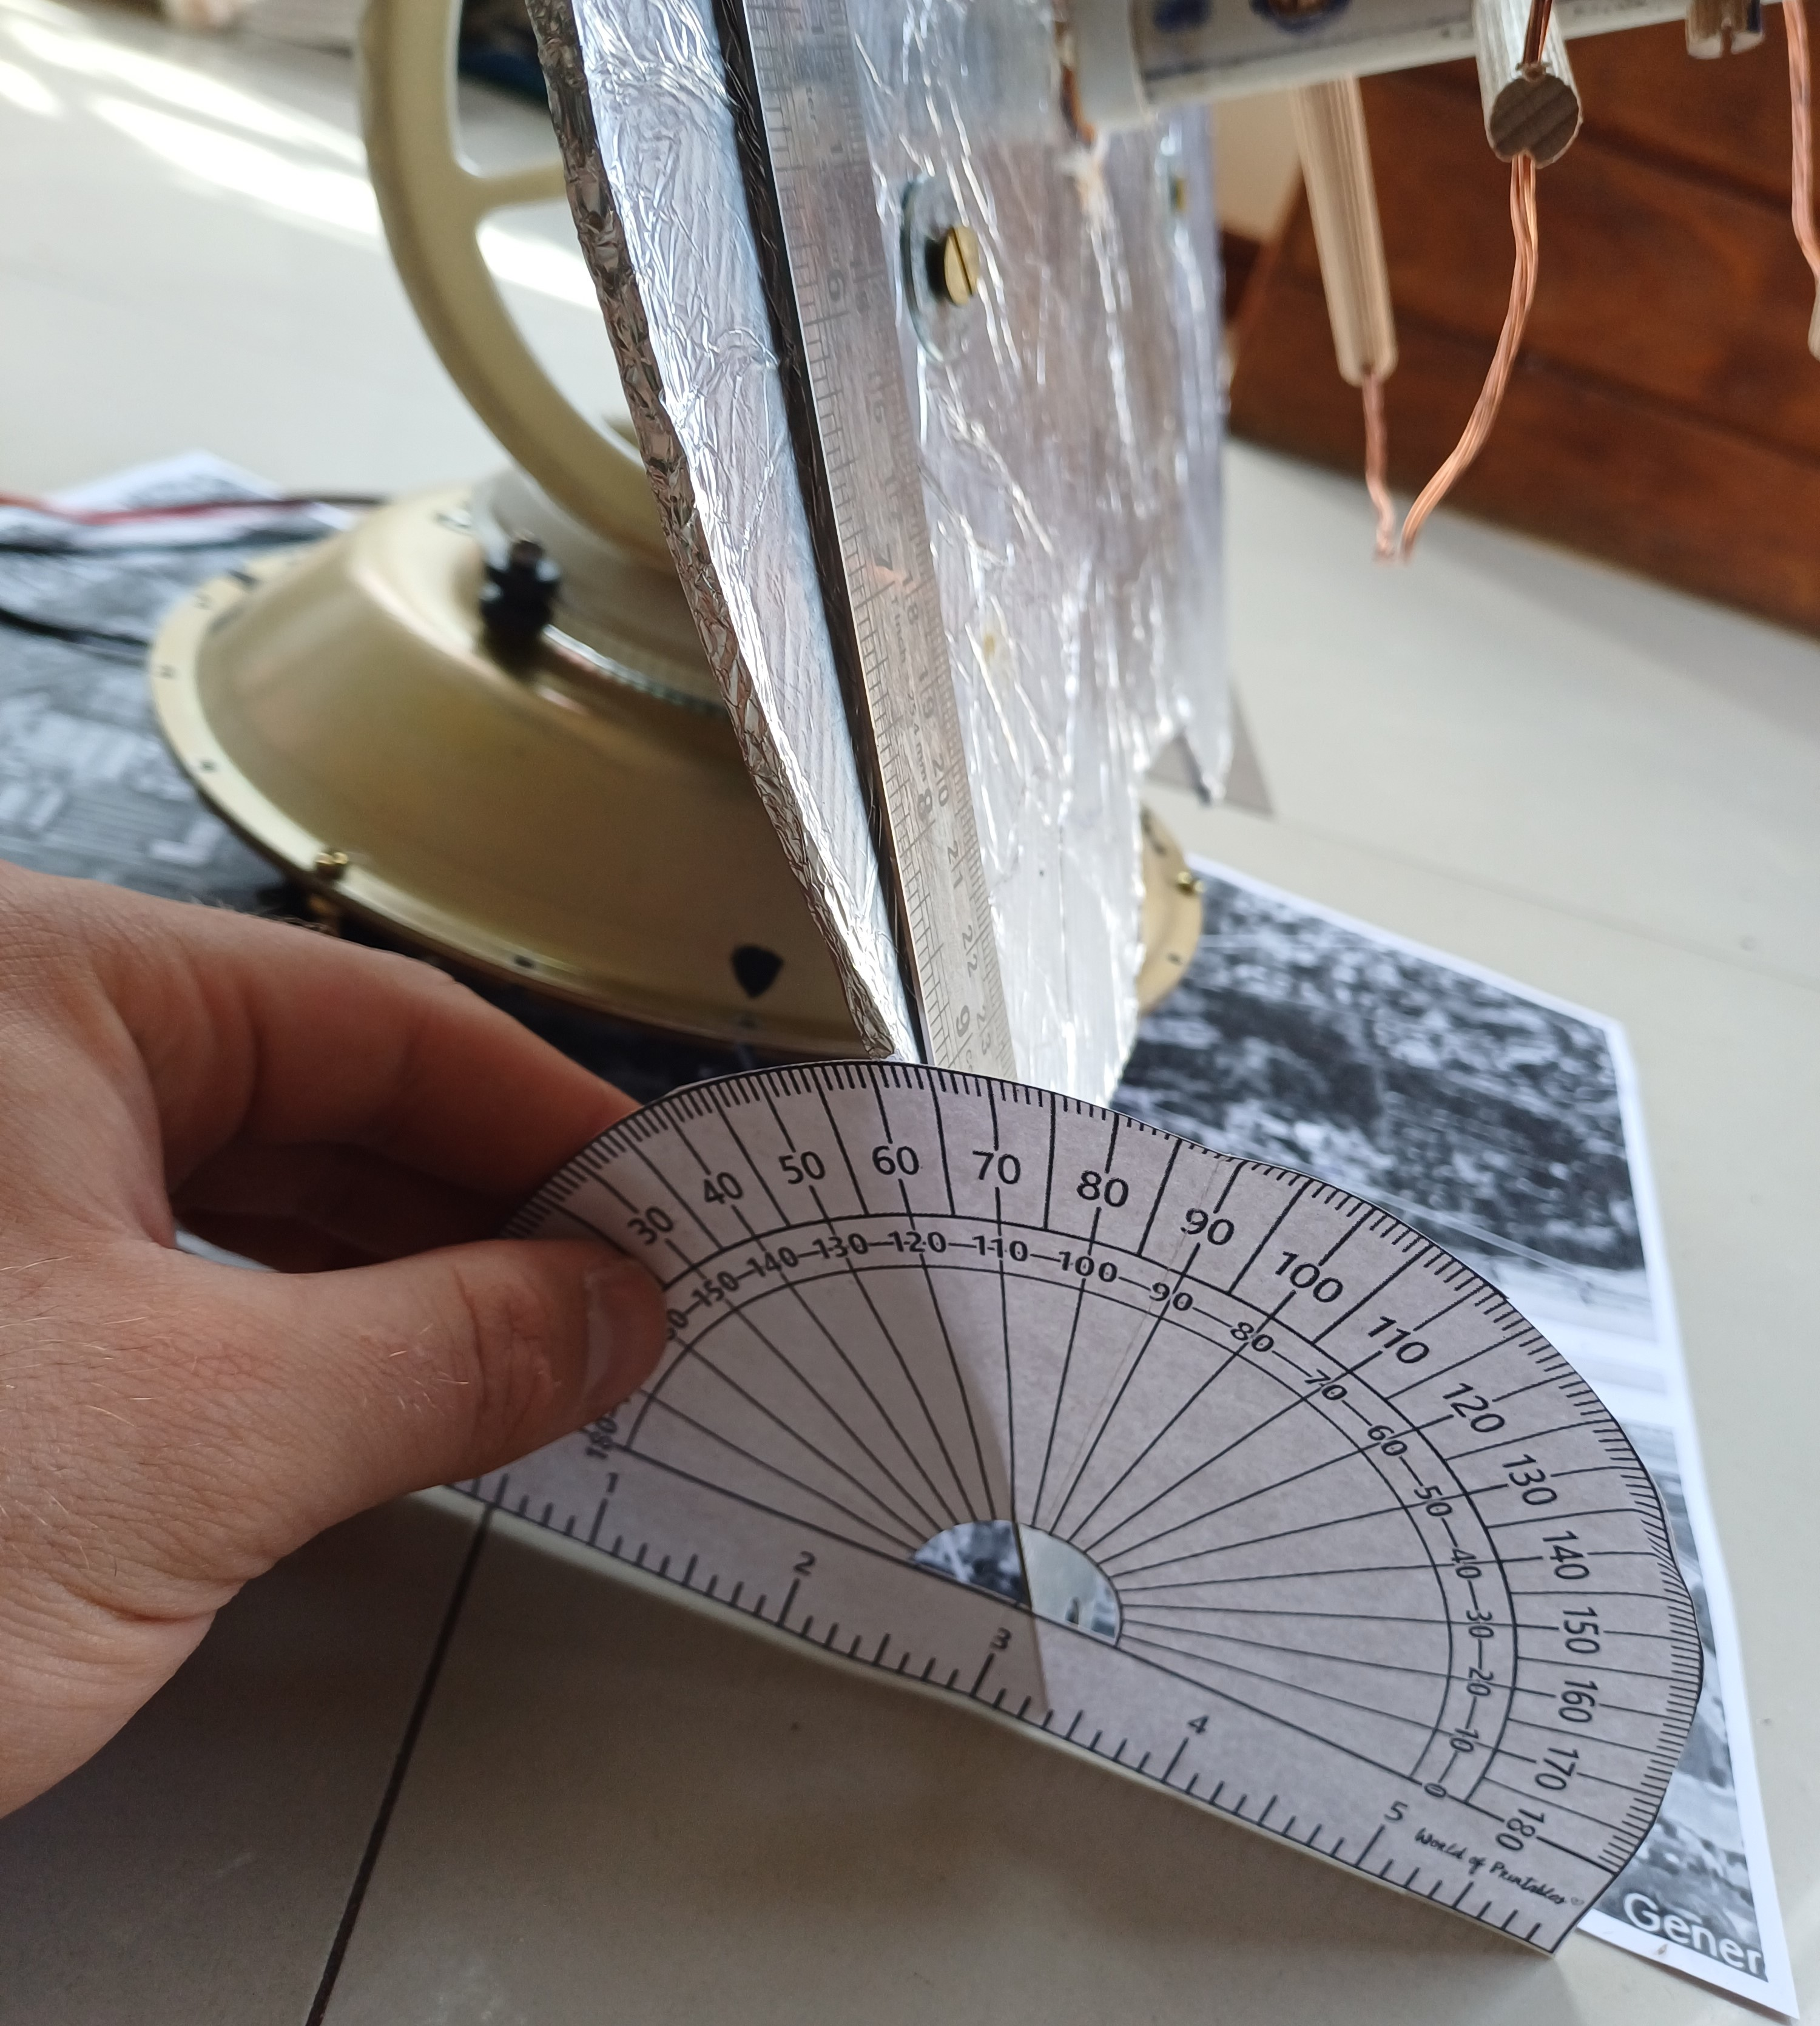
\includegraphics[width=0.75\linewidth]{pointingTestMeasurement}
    \caption{Open-Loop Pointing Test Elevation Angle Measurement}
    \label{fig:pointingTestMeasurement}
  \end{minipage}
\end{figure}

\begin{figure}[!htb]
  \centering
  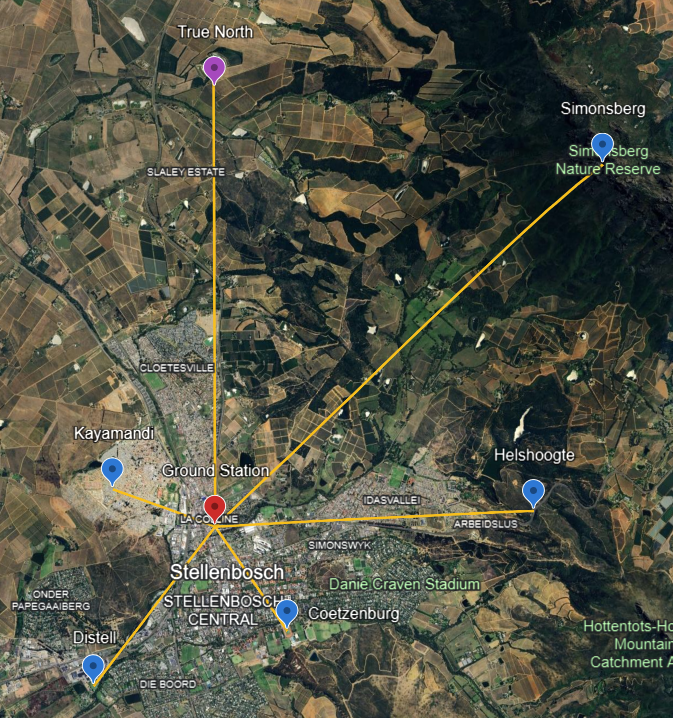
\includegraphics[width=0.4\textwidth]{pointingTestMap}
  \caption{Open-Loop Pointing Test Locations}
  \label{fig:pointingTestMap}
\end{figure}

\clearpage
\section{Range Tests}\label{sec:appendix_range}
\begin{figure}[!htb]
  \centering
  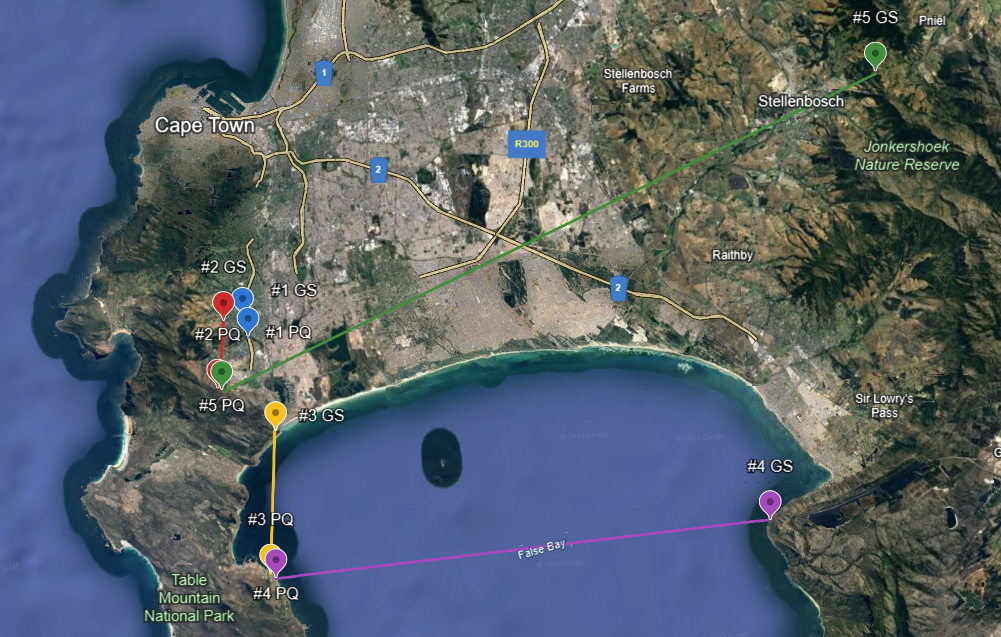
\includegraphics[width=0.8\textwidth]{rangeTests1}
  \caption{Range Tests Mapped Locations 1-5}
  \label{fig:rangeTests1}
\end{figure}
\begin{figure}[!htb]
  \centering
  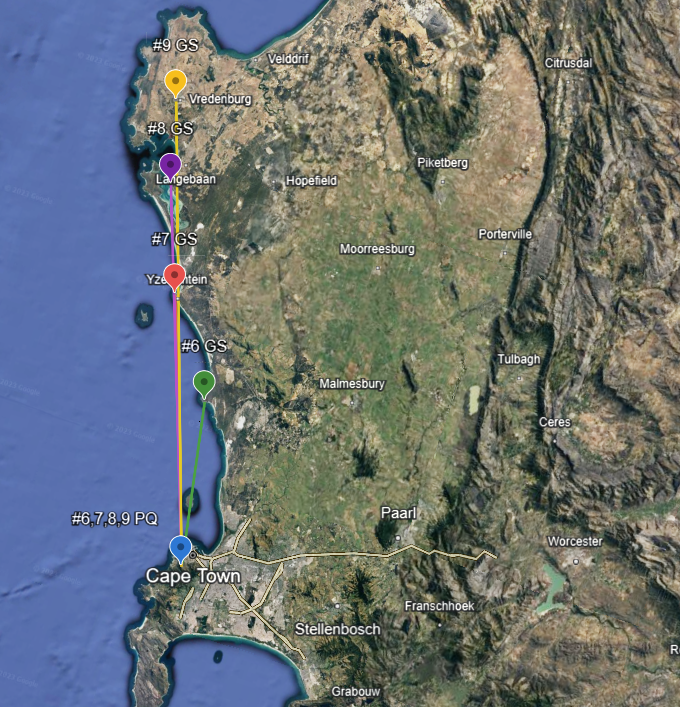
\includegraphics[width=0.65\textwidth]{rangeTests2}
  \caption{Range Tests Mapped Locations 6-9}
  \label{fig:rangeTests2}
\end{figure}
\begin{table}[!htb]
  \centering
  \renewcommand{\arraystretch}{1.2}
  \begin{tabular}{ |p{1cm}|c|p{4cm}|p{4cm}|p{3cm}| }
  \hline
  \textbf{Test No.}         & \textbf{Range}        & \textbf{GS Location}      & \textbf{PQ Location}      & \textbf{Comments} \\ 
  \hline
  1                         
  & 1.4 km  
  & Firgrove Way Bridge, Constantia
  & M3 Bridge near Keyser River
  & \\ \hline
  2
  & 4.6 km  
  & Firgrove Way Field, Constantia
  & Silvermine
  & Cloudy conditions \\ \hline
  3
  & 9.7 km  
  & Boyes Drive, Muizenberg
  & Windmill Beach, Simon's Town
  & \\ \hline
  4
  & 34.5 km  
  & Steenbras Lookout
  & Windmill Beach, Simon's Town
  & \\ \hline
  5
  & 49 km  
  & Tokara, Stellenbosch  
  & Silvermine Lookout Point
  & Optimal transmitter placement uncertainty \\ \hline
  6
  & 43 km  
  & Bokbaai
  & Table Mountain
  & \\ \hline
  7
  & 70 km  
  & Schaap Island, Yzerfontein
  & Table Mountain
  & \\ \hline
  8
  & 100 km  
  & Stompneus Lookout, Langebaan
  & Table Mountain
  & Sub-optimal transmitter placement (high multi-path effects observed) \\ \hline
  9
  & 122 km  
  & Rock near Frans Koch Ave, Vredenburg
  & Table Mountain
  & \\ \hline
  \end{tabular}
  \caption{Range Test Location Descriptions}
  \label{tab:rangeTestLocations}
\end{table}

\clearpage
\section{GUI}\label{sec:appendix_gui}
\begin{figure}[!htb]
  \centering
  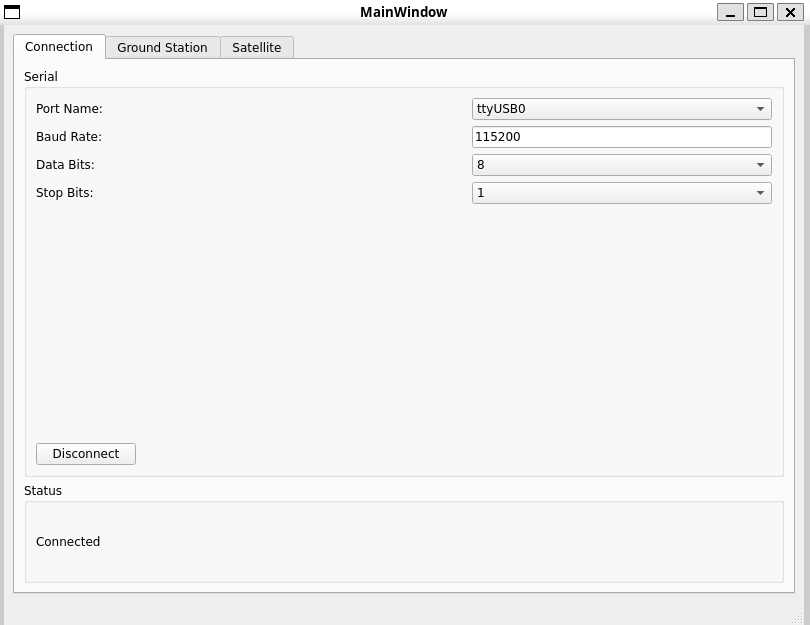
\includegraphics[width=0.8\textwidth]{guiConnection}
  \caption{GUI Output after Connecting to the Ground Station }
  \label{fig:guiConnection}
\end{figure}
\begin{figure}[!htb]
  \centering
  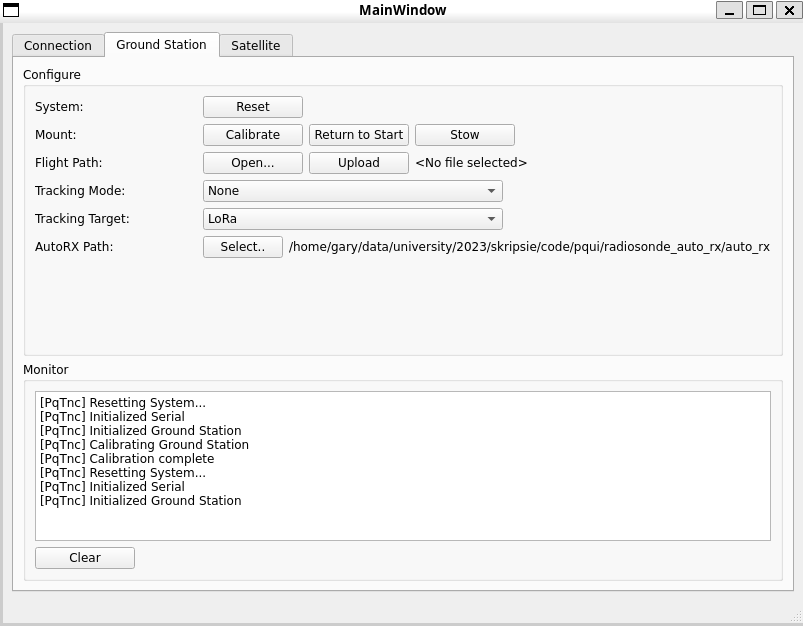
\includegraphics[width=0.8\textwidth]{guiCalibration}
  \caption{GUI Output after Reset, Calibration, and Reset Again}
  \label{fig:guiCalibration}
\end{figure}
\begin{figure}[!htb]
  \centering
  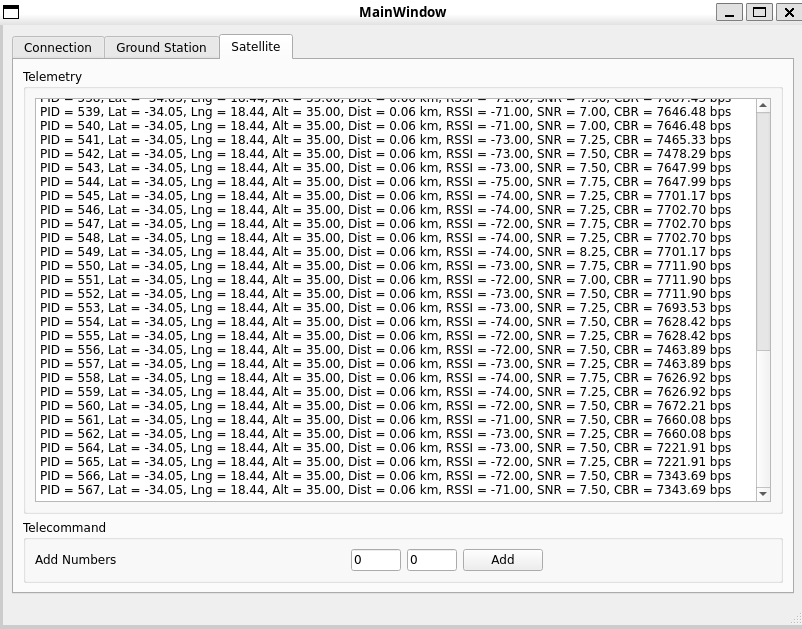
\includegraphics[width=0.8\textwidth]{guiTelemetry}
  \caption{GUI Output while Receiving Telemetry from LoRa Link}
  \label{fig:guiTelemetry}
\end{figure}